\documentclass[a4paper]{article}

\usepackage{INTERSPEECH2021}

\title{Sign Language Alphabet Translator Using Transfer Learning with Object Detection}
\name{Yi-Chuan Leuker, Agostino Calamia, Torsten Wolter}
\email{yi-chuan.leuker@fom-net.de, agostino.calamia@fom-net.de, torsten.wolter@fom-net.de}

\begin{document}

\maketitle
% 
\begin{abstract}
  Every country has its own sign language. There is no universal sign language in the world to help dead people communicate with others from other countries. This project focuses on developing a Sign Language Alphabet (SLA) translator that can play an important role by not only its interpretation but also helping deaf people to communicate with each other without learning a new sign language. In this project, the sign language used for training detective models is American sign language, and the detective models were imported from Pre-trained models for Transfer learning in the Keras library. The best six models, VGG16, ResNet50V2, MobileNet, MobileNetV2, DenseNet201, and Xception were selected by comparing the performance of the partial learning for further training of the full training dataset. After the training of the full training dataset, the six models were compared for accuracy and inference time and the result was MobileNet with an inference time as fast as 0.03 seconds and an accuracy of 99.68\%. The test dataset was further detected using this MobileNet model and the detected results were mapped to Turkish sign language images for translation.

  Index terms should be included as shown below.
\end{abstract}
\noindent\textbf{Index Terms}: sign language alphabet recognition, transfer learnings, object detection

\section{Introduction}
World Health Organization (WHO) projected that nearly 2.5 billion people in the world have hearing loss by 2050 and emphasized that sign language-related applications are essential tools for deaf people \cite{WHO2050}.

Instead of oral language using speaking and listening, Sign language is a form of visual communication through gestures, body movements and facial expressions. Sign language can be used for different purposes in different situations, but it is primarily designed for communication with the deaf. As it is more visually accessible to the deaf, sign language is a natural method of communication for the deaf and can express a wide range of meanings in the same way as spoken language; for example, American Sign Language is used by deaf people in the United States and partial provinces of Canada, British Sign Language is used by deaf people in the UK, French Sign Language in France, Japanese Sign Language in Japan and Chinese Sign Language in China.

Although there is no unified international sign language yet, the major sign language systems such as the USA, British, France and China have developed fingerspelling, also called "Sign Language Alphabet (SLA)." SLA represents the 26 common alphabets, A to Z, and local special letters using only hand gestures, mostly in difficult words such as personal names, place names and technical terms, etc. Additionally, it can also be used to facilitate easier communication when encountering issues with sign language dialects. 

In the past decade, deep learning has shown excellent performance in image recognition, enabling breakthroughs in sign language recognition technology. Many studies have used neural networks to convert static SLA signs into text or speech, using images of hand gestures as input, and the main approach includes data acquisition technique, static signs, classification with over 90\% accuracy of recognition \cite{wadhawan2021sign}. Moreover, Transfer Learning is one of the major milestones in Deep Learning for Object Detection. With Transfer Learning, pre-trained models have already been trained on a different task, therefore it is a short-cut that re-uses the pre-trained model and shorter the training process. This project aims to utilize pre-trained models from Transfer Learning with Object Detection in Keras and to apply static hand gesture images into different pre-trained model architecture to present a development of an SLA translator, which translates American SLA to Turkish SLA, thereby helping deaf people to communicate with each other without learning a new sign language. The remainder of this paper will include related work in the Sign language recognition research area, the problem statement found in the research, the objective of the project, and the methodology applied in the project. Afterwards, six pre-trained models, VGG16, ResNet50V2, MobileNet, MobileNetV2, DenseNet201, and Xception from Transfer Learning with Object Detection in Keras library are selected and trained as predictive models. The results of relevant inference time and accuracy are evaluated as performance to determine the best model for the use case. In end, the best model predicts ASL images using the test dataset, and the predicted results have a further mapping with Turkish SLA images.
  
\section{Related Work}
SLA translator is highly influenced by hand gesture recognition research using various devices for decades. There are two main approaches of sign language recognition: sensor-based or vision-based \cite{Cheok2019ARO}. The major difference between sensor-based and vision-based approaches is on the data acquisition phase. Sensor-based approaches utilize sensor instruments such as sensory glove to capture sign language, but such equipment was too complex and expensive to be widely actual used. On the other hand, vision-based approaches don't require complex facilities to acquire data, acquiring images or videos of the sign language through camera. For example, D., Cao et al.\cite{7301347} in 2015 developed sign language recognition by adapting Microsoft Kinect technology and used Random forest to successfully recognized static 24 American SLA with above 90\% accuracy. Furthermore, A., Joshi et al.\cite{8088212} presented a real-time automated American SLA translator that translates American SLA to English text by applying edge detection and cross-correlation methodologies, resulting in 94.23\% accuracy for alphabets. In recent years, Convolutional neural network (CNN) has become a common method applied in image recognition and classification. M., Taskiran et al.\cite{8441304} designed a real-time sign language system with an implementation of feature extraction and classifier based on a CNN structure, resulted in 98.05\% accuracy.

\section {Research question}
\subsection{Problem Statement}
The previous works showed great achievements in translating American SLA to texts by capturing images through cameras and using CNN for feature extraction and classification. However, an SLA translator from American SLA to other SLA is still not available today.

\subsection{Objective}
The goal for this research question aims to develop an SLA translator that use optimal transfer learning for object detection to recognise images of American SLAs and translate them into Turkish SLAs with images. For example, the American alphabet P in sign language is recognised and translated into the Turkish alphabet P in sign language. With sign language recognition, deaf people from different countries can communicate with each other without having to learn a new sign language.

\section{Methodology}

Figure \ref{fig:the proposed approach} shows the proposed approach to the ASL translator. The main approach to developing a translation from American SLA to other SLA is to build the best image recognition model that recognizes each English alphabet from the sign language with high accuracy. Instead of learning from scratch, Transfer learning with pre-trained models, which were already trained on a large benchmark image dataset, can save a lot of computation cost and help the performance. Kera applications provide a wide range of pre-trained models for deep learning such as VGG, ResNet, Xception, etc \cite{keras}. All the available pre-trained models will be applied into the first run training with the partial dataset to find out the Top 5 models with the highest accuracy of prediction. The top 5 models are further optimized and trained with all the training data to determine the best ASL recognition model. In the last phase, the results of prediction are mapping with Turkish ASL images.

\begin{figure}[h]
    \centering
    \caption{The proposed approach for the sign language translator}
	\label{fig:the proposed approach}
    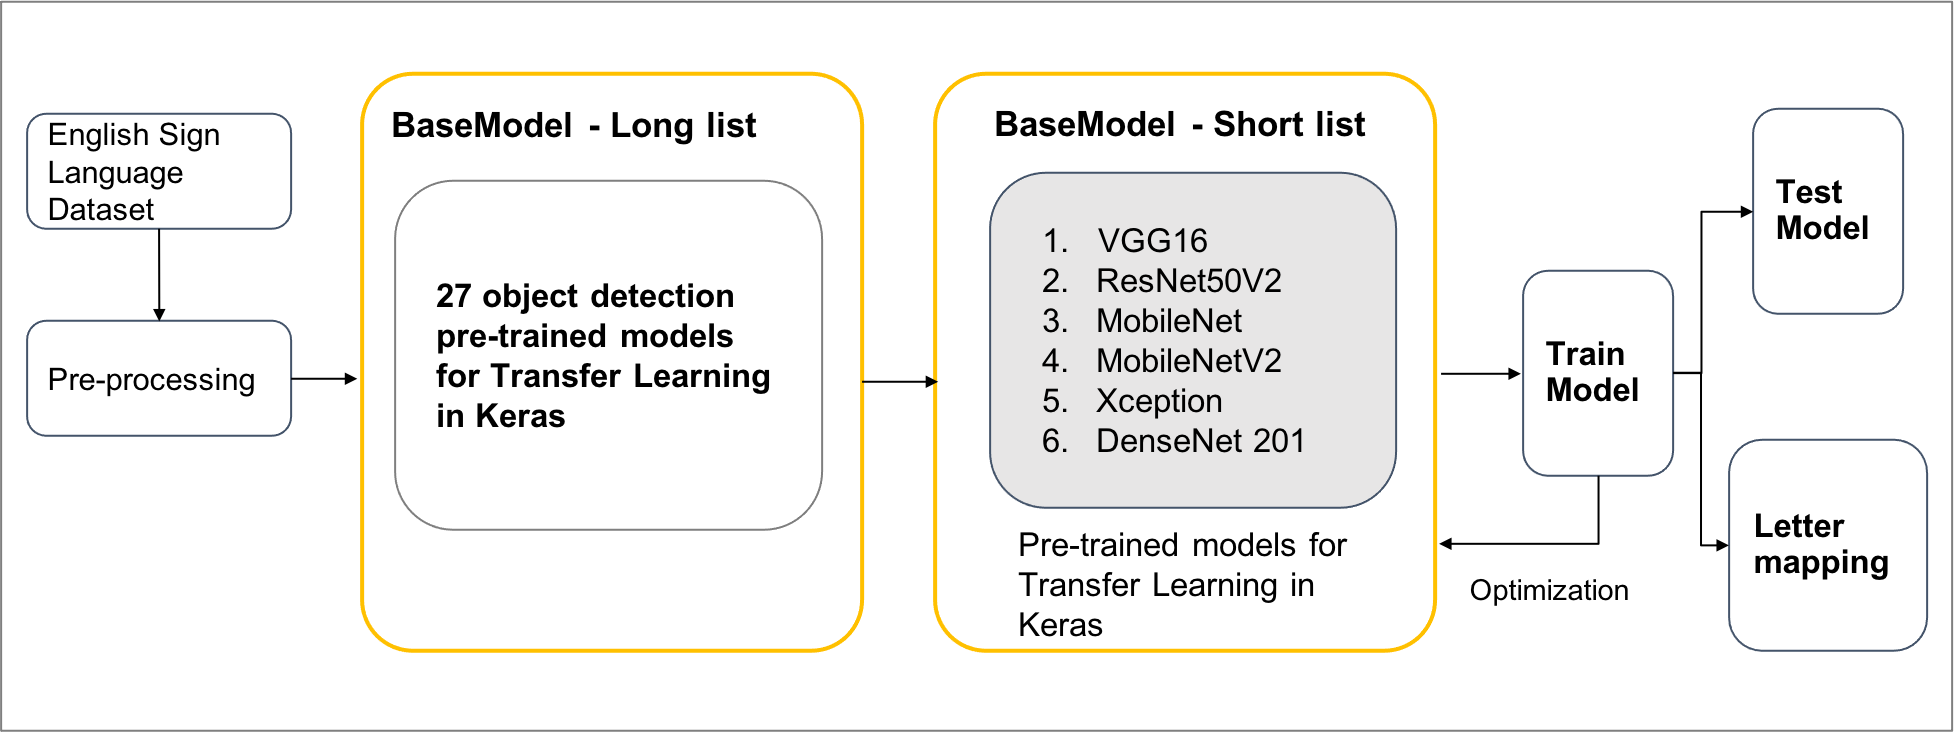
\includegraphics[width=\linewidth]{figures/The approach}
\end{figure}


\subsection{Dataset}
The American ASL dataset is collected from Kaggle. The dataset contains 87,000 images with 26 Englich alphabets and 3 extra signs, which are delete, space, and nothing. All the images are equally distributed to the 29 signs. In other words, each sign has 4,300 images. The whole dataset is split into training and test dataset. Training dataset is 80\% of the data, and the rest data belongs to the test dataset. 


\subsection{Image preprocessing}

\subsection{Transfer learning models}
One of the main benefits of using transfer learning is to make use of previously trained models and save computational cost (CC) for basic tasks like the removal of background. It may also be used when the training data is sparse. For the detection of American SLA we may use (to a degree) any pre-trained model for object detection on our dataset of American SLA signs even if they are limited in count and quality, as they only make the last layer of our final model.

To determine, whether a model may be suitable for our application, we use all of the models and its variants available in Keras\cite{keras}, as shown in Table~\ref{tab:keras_models}. The \textit{Avg. Top-5 Accuracy} in the table refers to the average accuracy of all variants combined.
\begin{table}[th]
    \caption{Keras Applications}
    \label{tab:keras_models}
    \centering
    \begin{tabular}{@{}lrcl@{}}
    \toprule
    Name         & \multicolumn{1}{l}{\begin{tabular}[c]{@{}l@{}}Avg. Top-5\\ Accuracy\end{tabular}} & \multicolumn{1}{l}{Total} & \begin{tabular}[c]{@{}l@{}}Variants\\ (*=Model)\end{tabular}                         \\ \midrule
    Xception     & 0.945                                                                             & 1                         & *                                                                                    \\
    VGG          & 0.901                                                                             & 2                         & *16, *19                                                                             \\
    ResNet       & 0.931                                                                             & 6                         & \begin{tabular}[c]{@{}l@{}}*50, *101, *152,\\  *50V2, *101V2,\\  *152V2\end{tabular} \\
    Inception    & 0.945                                                                             & 2                         & *V3, *ResNetV2                                                                       \\
    MobileNet    & 0.898                                                                             & 2                         & *, *V2                                                                               \\
    DenseNet     & 0.930                                                                             & 3                         & *121, *169, *201                                                                     \\
    NASNet       & 0.940                                                                             & 2                         & *Mobile, *Large                                                                      \\
    EfficientNet & -                                                                                 & 8                         & \begin{tabular}[c]{@{}l@{}}*B0, *B1, *B2,\\  *B3, *B4, *B5,\\  *B6, *B7\end{tabular} \\ \bottomrule
    \end{tabular}
\end{table}

In order to determine, which of the above stated models we will further evaluate and possibly optimize, we train each of the Keras models in an experimental setup. The experimental training is defined by:
\begin{enumerate}
    \item Training with 5\% of the dataset (~4.300 images, equally distributed to the 29 targets), with a 80/20 Train-Test-Split
    \item 10 Epochs of Training
    \item No Early Stopping
\end{enumerate}

The results will focus on two key indicators: accuracy on our dataset and training time.

The following subsections will give a brief introduction of the most relevant model families and how they differ.

\subsubsection{VGG16}
The VGG models are one of the earlier computer vision models an were introduced in 2015 by Simonyan and Zisserman which showed that using deep architectures with rather small filters can be superior to other models at that time\cite{simonyan2015deep}. VGG represents a classical convolutional neural network which takes an 224x224x3 (width x height x channels) input pictures and passes it to multiple convolutional layers, pooling layers and activation functions to a fully connected final layer for classification. It includes in total 16 layers with weights and is shown in figure \ref{fig:vgg16}.

\begin{figure}
  \centering
  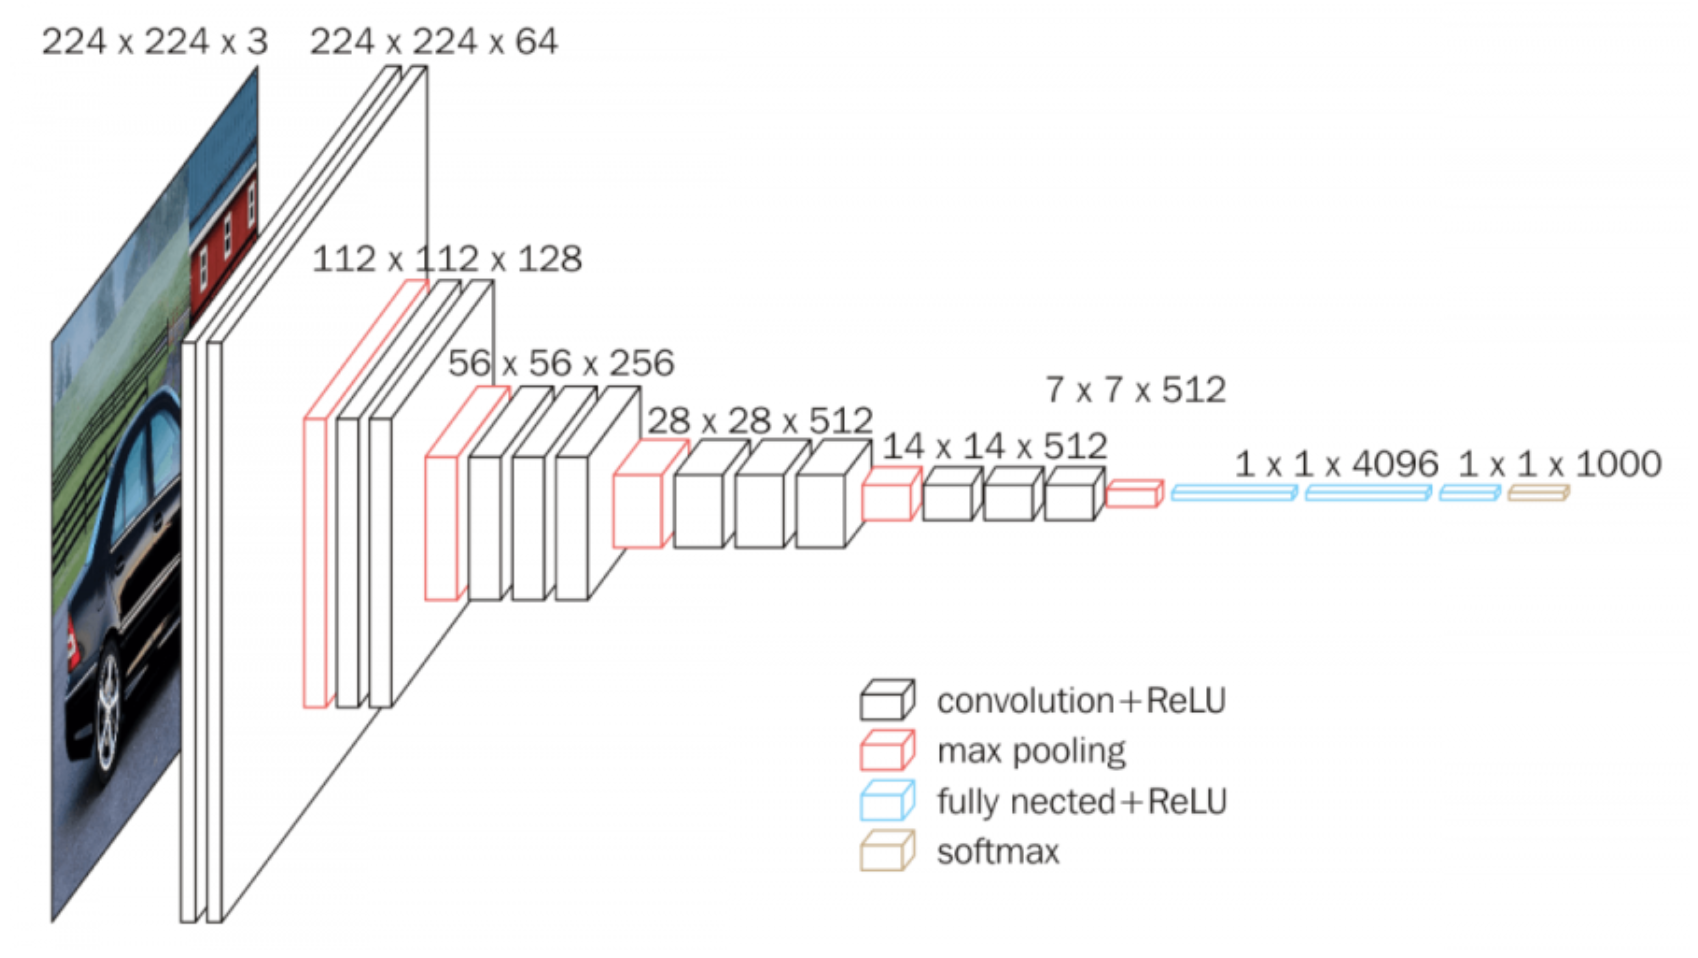
\includegraphics[width=\linewidth]{figures/vgg16.png}
  \caption{VGG16 architecture}
  \label{fig:vgg16}
\end{figure}

The tremendous change compared to previous convolutional neural networks is that the used filters and layers have the same size and parameters such as only ReLu as activation function\cite{simonyan2015deep}. This newly introduced simplicity paired with a relatively deep architecture led to unique results in the ILSVRC-2012 and ILSVRC-2013 competitions compared to the previous state-of-art AlexNet. On top of that is was shown that the model had a strong ability to generalise over multiple datasets and still achieve a top 5 performance. The authors of the network structured it in a way that it is possible to move from 16 layers to 19 layers for even better results.

\subsubsection{ResNet50V2}

\subsubsection{MobileNet}

\subsubsection{MobileNetV2}

\subsubsection{DenseNet 201}

\subsubsection{Xception}

\section{Results}\label{chapter_results}
In order to find the most suitable algorithm for translating a live input stream of American SLA to any other suitable SLA (sharing the same alphabet) in a real-world application, the algorithm needs to excel in two main aspects: accuracy and inference time. A third factor that may come into question here is the training time, as the computational cost may accumulate when further improving the model in the future.

\subsection{The long list}\label{chapter_long}
As mentioned in chapter \ref{chapter_models} the long list contained 27 pretrained models. Due to the limited availability of computational resources, the models on the list as per table \ref{tab:keras_models} (including all variants) were trained in an experimental setup to determine which models are suitable for full training. The goal was to use these pretrained models and only train the last layer to enable the detection of SLA in sources such as webcam feeds, videos or images.

The experimental setup was trained on a consumer pc, with a 3.8 Ghz 6-core CPU, a \textit{GeForce GTX 1060} GPU and 32GB of RAM. The results mainly focus on two aspects in order to decide which models may be suitable for the full training: training time and accuracy. As shown in Fig. \ref{fig:long_list_acc} some of the models already have high accuracy with a minified training.

\begin{figure}[h]
    \centering
    \caption{Accuracy on long list training}
	\label{fig:long_list_acc}
    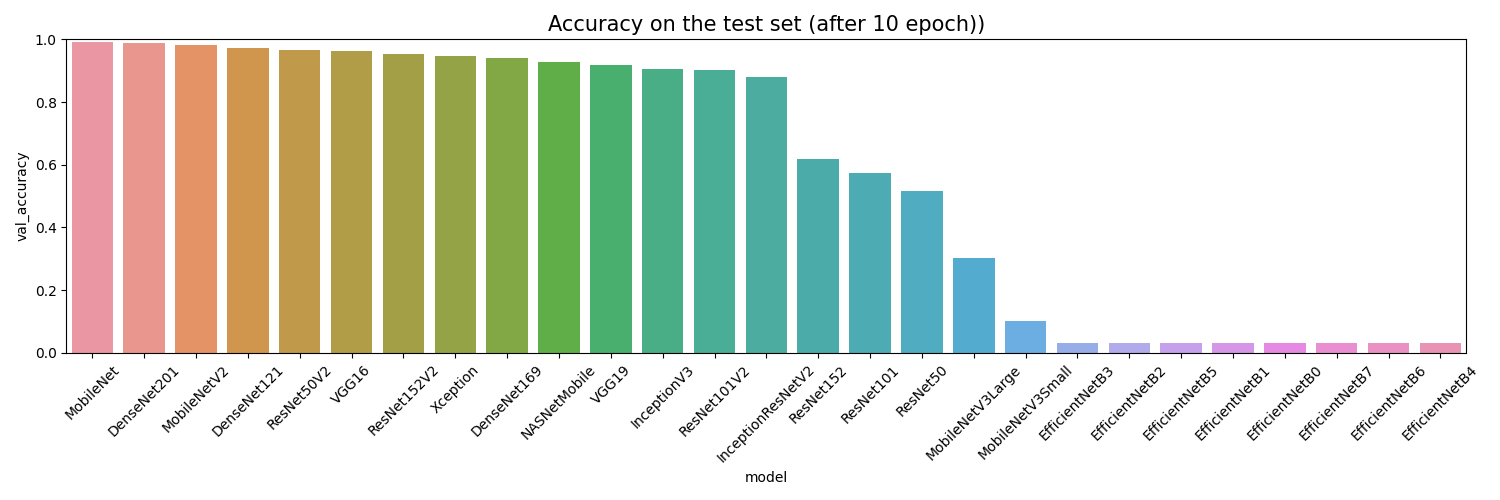
\includegraphics[width=\linewidth]{figures/long_val_accuracy.png}
\end{figure}

While models as \textit{DenseNet} seem to have good results with all variants, others like \textit{ResNet} have a high variety; accuracy ranges from ~55\% (\textit{ResNet50}) to ~98\% \textit{ResNet50V2}. The \textit{EfficientNet} with all its variants has an accuracy below 10\% and will not move forward.

\begin{figure}[h]
    \centering
    \caption{Training time on long list training}
	\label{fig:long_list_time}
    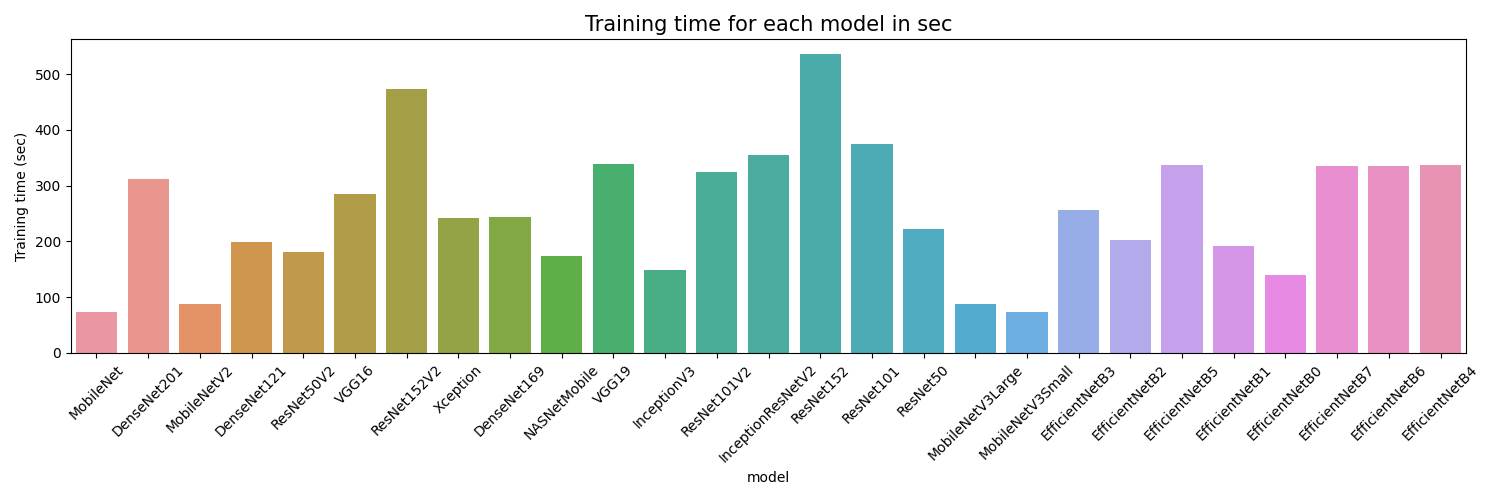
\includegraphics[width=\linewidth]{figures/long_training_time.png}
\end{figure}

Fig. \ref{fig:long_list_time} shows the time that was needed to train the models with the reduced dataset for 10 epochs without early stopping. While it shows a wide range, the times train not too long at all. Therefore, the training time will not be the main factor in deciding which model we should move forward with.

When deploying the model in a real-time environment, such as live detection via a webcam, another factor comes into play: the inference time. As described in chapter \ref{chapter_models}, the models differ fundamentally in their architecture. At this point, it is uncertain how the architectural structure will affect the inference time of a fully trained model. Therefore we decided to move forward with the best performing model from each architecture described in chapters \ref{chapter_vgg16} to \ref{chapter_xception}. In addition to the top 5 models, we decided to add \textit{MobileNetV2} as well, as it seemed interesting why the newer version of the model did perform worse than the old one. Table \ref{tab:results:long} contains all models that will be used for full training.

\begin{table}[th]
    \caption{Short List candidates}
    \label{tab:results:long}
    \centering
    \begin{tabular}{lll}
    \hline
    Name        & Acc.   & \begin{tabular}[c]{@{}l@{}}Time\\ (seconds)\end{tabular} \\ \hline
    MobileNet   & 0.9957 & 82                                                       \\
    MobileNetV2 & 0.9756 & 165                                                      \\
    DenseNet201 & 0.9842 & 328                                                      \\
    ResNet50V2  & 0.9239 & 178                                                      \\
    Xception    & 0.9698 & 238                                                      \\
    VGG16       & 0.9382 & 286                                                      \\ \hline
    \end{tabular}
\end{table}

\subsection{The short list}
For the short list produced in chapter \ref{chapter_long} the training was slightly adapted. In contrast to the training of the long list, Early Stopping with a \textit{patience=1} was implemented in order to stop the training after 1 epoch without any improvement of the loss rate to avoid an overfit. Since no further knowledge for expected epochs needed was given, a maximum of 50 epochs was configured. Table \ref{tab:results:short} shows the result of the training.

\begin{table}[th]
    \caption{Short List Results}
    \label{tab:results:short}
    \centering
    \begin{tabular}{@{}lllll@{}}
    \toprule
    Name        & Acc.   & Change \% & \begin{tabular}[c]{@{}l@{}}Time\\ (seconds)\end{tabular} & \begin{tabular}[c]{@{}l@{}}stopped\\ at\end{tabular} \\ \midrule
    MobileNet   & 0.9921 & -0.36     & 160                                                      & 2                                                      \\
    MobileNetV2 & 0.9900 & +1.48     & 385                                                      & 4                                                      \\
    DenseNet201 & 0.9905 & +0.64     & 1058                                                     & 3                                                      \\
    ResNet50V2  & 0.9840 & +6.51     & 578                                                      & 3                                                      \\
    Xception    & 0.9820 & +1.26     & 746                                                      & 3                                                      \\
    VGG16       & 0.9960 & +6.16     & 1975                                                     & 7                                                      \\ \bottomrule
    \end{tabular}
\end{table}

As we can see, the results did not significantly change in comparison to the minified setup, reflected by the \textit{Change \%} column. Although using the full dataset instead of only 10\%, the training time did not increase the expected folds due to the early stopped training. As in the minified training, \textit{MobileNetV2}'s accuracy remains lower than its predecessor \textit{MobileNet}, even with a later stopped training. At this point, it still remains unclear why this can be observed.

\subsection{Inference Time}
As mentioned above, training time and accuracy are not the only factors when choosing a suitable model for a real-time application. Accuracy is high across all fully trained models, and while training time differs within the short list results, it can be disregarded as the total times are relatively short, even when the training runs on a consumer machine. Training time also does not accumulate due to the early stopping mechanism. In order to select the best model, the inference time is the crucial value as it determines how many frames (predictions) the model can handle per second, a key factor for a real-time application.
The inference time was measured with the above saved models. All models executed the predictions on the same initially randomly selected 544 images with a batch size of \begin{math}n=32\end{math}. The process was repeated 10 times with different randomly selected images.

\begin{figure}[h]
    \centering
    \caption{Avg. Inference in Seconds}
	\label{fig:result:inference}
    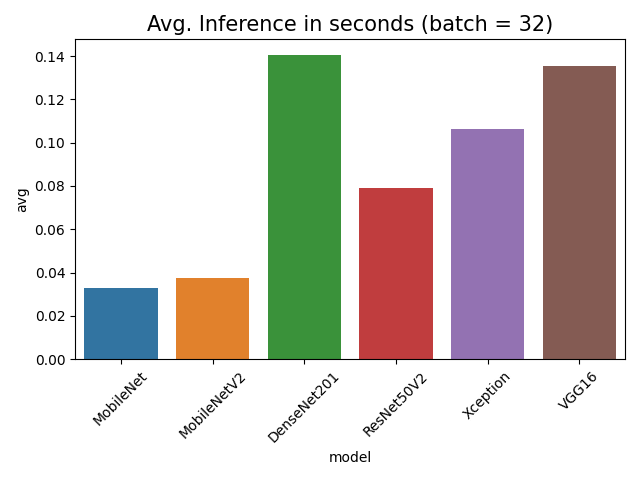
\includegraphics[width=\linewidth]{figures/inference.png}
\end{figure}

The results visualized in Fig. \ref{fig:result:inference} show that only \textit{MobileNet} and \textit{MobileNetV2} have near real-time capabilities. While a prediction time of 0.14 seconds (\textit{DenseNet201}, Fig. \ref{fig:result:inference}) does seem acceptable to the human eye, it translates to approx. 7 predictions per second. Given that the human eye can detect meaning in images within 13ms\cite{Potter2014} (approx. 75 frames per second (fps)) and videos have a minimum framerate of 23.97 fps to appear smooth and fluent, 7 predictions (frames) per second will not lead to an acceptable user experience. Therefore only the \textit{MobileNet} and \textit{MobileNetV2} should be considered for real-time applications, as the inference time of 0.03 seconds leads to a framerate of approx. 33 fps.

\subsection{Shipping production-ready Model}
The final implementation of the trained model is up to the user. Each trained model is saved as a portable \textit{Tensorflow} file and can be used to implement a real-time detection via \textit{OpenCV}, for example. In order to confirm the usability of the model, we implemented an application, which takes static images as an input and outputs them according to the image of a predefined SLA dataset of another language. 

The target SLA for the sample implementation was the Turkish Sign Language (TSL), and the \textit{MobileNet} model was used. As any real-time application would have, the dimensions and resolution of the input data differed from the images used in training. Fig. \ref{fig:result:translation} shows a sample output for the translation of the left sign (ASL Letter D), the predicted sign and the according to output image for the TSL.

\begin{figure}[h]
    \centering
    \caption{Sample Translation from ASL to TSL, Letter D}
	\label{fig:result:translation}
    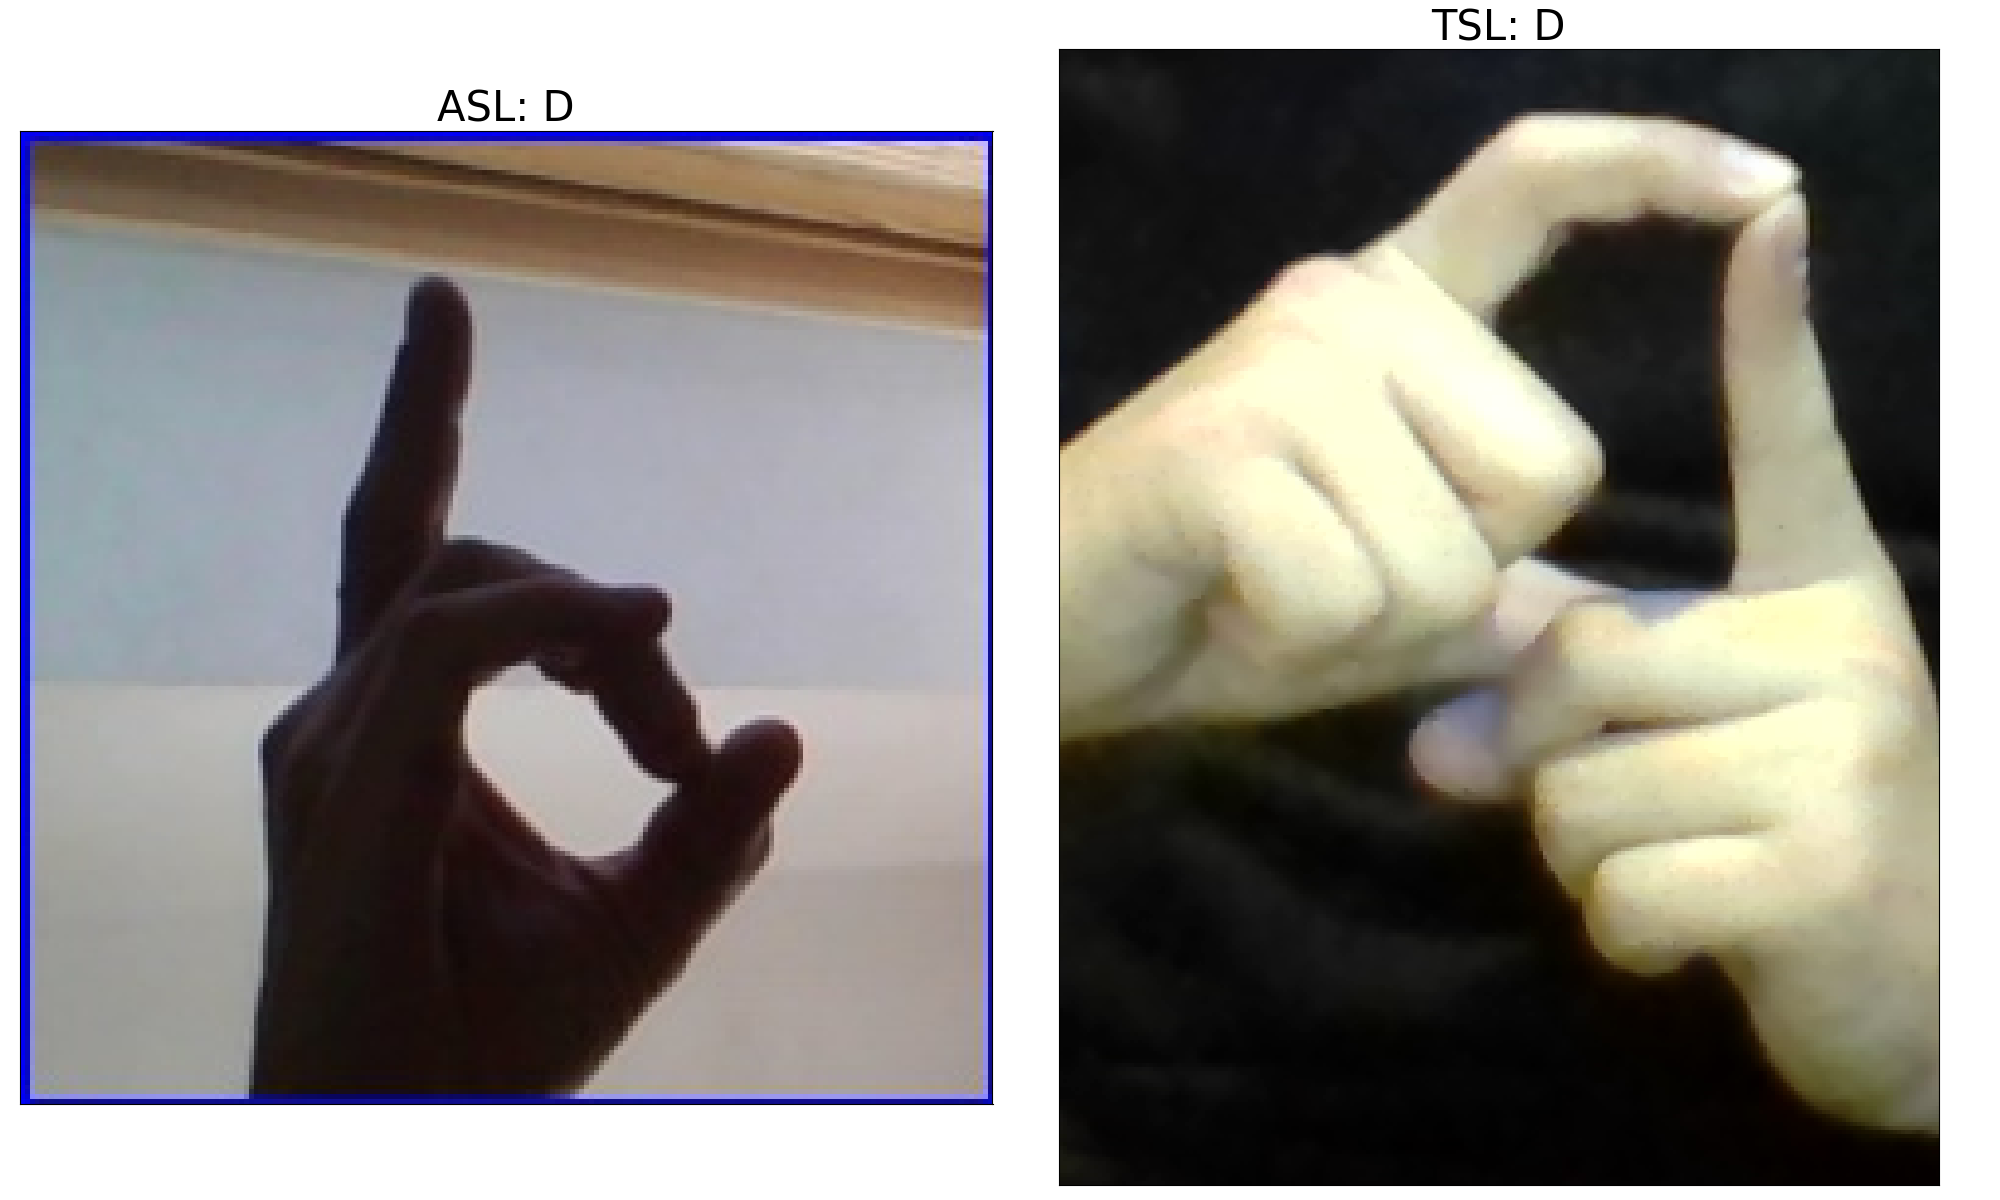
\includegraphics[width=\linewidth]{figures/sample_translate_D_tur.png}
\end{figure}


\subsection{Equations}

Equations should be placed on separate lines and numbered. Examples of equations are given below. Particularly,
% 
\begin{equation}
  x(t) = s(f_\omega(t))
  \label{eq1}
\end{equation}
% 
where \(f_\omega(t)\) is a special warping function
% 
\begin{equation}
  f_\omega(t) = \frac{1}{2 \pi j} \oint_C 
  \frac{\nu^{-1k} \mathrm{d} \nu}
  {(1-\beta\nu^{-1})(\nu^{-1}-\beta)}
  \label{eq2}
\end{equation}
% 
A residue theorem states that
% 
\begin{equation}
  \oint_C F(z)\,\mathrm{d}z = 2 \pi j \sum_k \mathrm{Res}[F(z),p_k]
  \label{eq3}
\end{equation}
% 
Applying (\ref{eq3}) to (\ref{eq1}), it is straightforward to see that
% 
\begin{equation}
  1 + 1 = \pi
  \label{eq4}
\end{equation}

Finally we have proven the secret theorem of all speech sciences. No more math is needed to show how useful the result is!

\begin{figure}[t]
  \centering
  \includegraphics[width=\linewidth]{figure.pdf}
  \caption{Schematic diagram of speech production.}
  \label{fig:speech_production}
\end{figure}



\subsection{Multimedia files}

The INTERSPEECH organizing committee offers the possibility to submit multimedia files. These files are meant for audio-visual illustrations that cannot be conveyed in text, tables and graphs. Just like you would when including graphics, make sure that you have sufficient author rights to the multimedia materials that you submit for publication. The proceedings media will NOT contain readers or players, so be sure to use widely accepted file formats, such as MPEG, Windows WAVE PCM (.wav) or Windows Media Video (.wmv) using standard codecs.

Your multimedia files must be submitted in a single ZIP file for each separate paper. Within the ZIP file you can use folders and filenames to help organize the multimedia files. In the ZIP file you should include a TEXT or HTML index file which describes the purpose and significance of each multimedia file. From within the manuscript, refer to a multimedia illustration by its filename. Use short file names without blanks for clarity.

The ZIP file you submit will be included as-is in the proceedings media and will be linked to your paper in the navigation interface of the proceedings. Causal Productions (the publisher) and the conference committee will not check or change the contents of your ZIP file.

Users of the proceedings who wish to access your multimedia files will click the link to the ZIP file which will then be opened by the operating system of their computer. Access to the contents of the ZIP file will be governed entirely by the operating system of the user's computer.

\subsection{Page numbering}

Final page numbers will be added later to the document electronically. \emph{Do not make any footers or headers!}


\subsection{References}
The reference format \cite{Wiederhofer2017} is the standard IEEE one. References should be numbered in order of appearance, for example \cite{Davis80-COP}, \cite{Rabiner89-ATO}, \cite[pp.\ 417--422]{Hastie09-TEO}, and \cite{YourName21-XXX}.

\subsection{Abstract}

The total length of the abstract is limited to 200 words. The abstract included in your paper and the one you enter during web-based submission must be identical. Avoid non-ASCII characters or symbols as they may not display correctly in the abstract book.

\subsection{Author affiliation}

Please list country names as part of the affiliation for each country.

\subsection{Number of authors in the author list}

The maximum number of authors in the author list is twenty. If the number of contributing authors is more than twenty, they should be listed in a footnote or in acknowledgement section, as appropriate.

\subsection{Submitted files}

Authors are requested to submit PDF files of their manuscripts. You can use commercially available tools or for instance http://www.pdfforge.org/products/pdfcreator. The PDF file should comply with the following requirements: (a) there must be no PASSWORD protection on the PDF file at all; (b) all fonts must be embedded; and (c) the file must be text searchable (do CTRL-F and try to find a common word such as ``the''). The proceedings editors (Causal Productions) will contact authors of non-complying files to obtain a replacement. In order not to endanger the preparation of the proceedings, papers for which a replacement is not provided in a timely manner will be withdrawn.

\section{Discussion}

This is the discussion. This is the discussion. This is the discussion. Is there any discussion?

Lorem ipsum dolor sit amet, consectetur adipiscing elit. Cras consequat mollis odio, nec venenatis enim auctor sed. Integer tincidunt fringilla lectus eget condimentum. In eget sapien id eros dapibus interdum vel ac quam. Aenean vitae rutrum erat. Aenean et risus pharetra, lacinia augue ut, fermentum ante. Integer dui arcu, interdum at ornare a, faucibus quis est. Mauris quis quam felis. Etiam pulvinar massa et turpis lacinia, eu posuere mi iaculis. Fusce at velit quis leo dignissim porttitor.

Fusce ut nunc eu sapien venenatis finibus a vel ligula. Pellentesque habitant morbi tristique senectus et netus et malesuada fames ac turpis egestas. Ut quam eros, volutpat at gravida consectetur, rutrum ut leo. Aenean cursus euismod feugiat. Cras hendrerit, ligula eu feugiat malesuada, neque turpis auctor lacus, sit amet accumsan neque orci a quam. Mauris suscipit ultrices mattis. Nulla at interdum metus, id pharetra diam. Curabitur at vestibulum sem, sed elementum massa. Donec iaculis et arcu ut rutrum. Fusce gravida, mauris porta volutpat eleifend, enim mauris eleifend orci, eu ultrices leo purus vitae metus. In pretium dolor ut magna dictum, at imperdiet lectus porta.

Quisque mollis lectus id risus pretium mattis. Morbi scelerisque posuere est, id efficitur urna luctus non. Praesent quam lacus, facilisis id ante eu, vehicula maximus ex. Nullam mollis in arcu vitae efficitur. Aliquam molestie eleifend ante, in pretium velit ultrices ac. Etiam laoreet nec sem non pulvinar. Integer ligula felis, interdum non lacus id, malesuada imperdiet turpis.

Aenean sit amet volutpat nisi. Aliquam eu erat quis tortor ultrices laoreet. Vivamus fermentum semper metus, non faucibus libero euismod vitae. Sed efficitur porta congue. Aenean in faucibus nisi. Donec suscipit augue vitae orci consequat, sit amet aliquet felis varius. Duis efficitur lacinia dolor sit amet lobortis. Curabitur erat sapien, molestie nec nisi eu, dignissim accumsan ipsum. Fusce id nibh nec risus dictum posuere in ac magna. Donec malesuada massa sed erat lacinia cursus. Suspendisse ornare augue nec volutpat consequat.

Vestibulum et vulputate nisi, a malesuada mi. Nam pellentesque arcu sapien, at placerat odio imperdiet ut. Curabitur nec venenatis tellus, vel aliquet nisi. Curabitur vel ligula sit amet metus auctor pretium. Nullam nulla mi, blandit a mattis id, vulputate sit amet enim. Proin mollis fringilla dictum. Proin lacinia orci purus.

Curabitur porttitor bibendum dolor, nec consectetur sapien pulvinar id. Donec eleifend, est vel dignissim pretium, tortor augue euismod nunc, id fermentum erat felis ac neque. Morbi id lectus ultricies, rutrum justo eu, sollicitudin risus. Suspendisse lobortis efficitur nisi sit amet pellentesque. Ut eget augue at mi aliquet mattis. Proin et feugiat erat, sit amet sodales eros. Integer sed elit quis est mattis ullamcorper. Pellentesque lectus nisi, vulputate a imperdiet tincidunt, auctor nec orci. Pellentesque sagittis nisl orci, vitae placerat massa lacinia nec. Sed egestas magna sed augue sollicitudin luctus. Praesent interdum bibendum tortor, eu porta purus. Aliquam convallis velit id mi fermentum, sed ornare eros cursus.

Quisque congue leo a fringilla pharetra. Phasellus sed tempor est, sed auctor purus. Morbi vel lacus ullamcorper, auctor mauris id, pulvinar lorem. Suspendisse potenti. Nam porta, purus non eleifend bibendum, erat metus pellentesque elit, non luctus nibh nunc ornare nisl. Sed rutrum lacinia nisi ac suscipit. Curabitur non blandit augue. Integer viverra, ipsum vel molestie euismod, sem quam tempus massa, eget efficitur ante turpis non metus. Quisque efficitur posuere velit in iaculis. Cras imperdiet varius urna vitae vestibulum. Donec accumsan eget nisi sed pellentesque. Vestibulum id quam ut urna volutpat ullamcorper gravida sit amet libero. Aliquam bibendum, ligula vitae porta malesuada, arcu diam congue erat, a pharetra diam sem vulputate tortor. Etiam luctus iaculis leo cursus tristique.

Mauris mattis sem dolor, sit amet ullamcorper arcu tincidunt ac. Vestibulum at blandit tortor. Quisque bibendum congue leo, vitae eleifend massa. Vestibulum vitae odio elit. Lorem ipsum dolor sit amet, consectetur adipiscing elit. Ut sagittis quam vel felis ornare, in gravida felis tempor. Donec molestie dui quis leo venenatis blandit. Nunc sit amet finibus metus. Cras ut lectus ex.

Suspendisse commodo libero vel leo tincidunt, a tempus mauris porta. Integer varius eros ac sapien lacinia vehicula. Donec porttitor, lacus faucibus rhoncus venenatis, neque quam imperdiet nunc, id consectetur metus purus quis sapien. Phasellus interdum nulla vel euismod posuere. Vestibulum finibus magna vel finibus mollis. Curabitur mollis turpis tortor, hendrerit vulputate justo egestas quis. Nam dignissim luctus leo non elementum. Phasellus a metus at leo malesuada bibendum. Mauris quis eleifend magna, nec vehicula ex. Donec venenatis urna fermentum commodo vehicula. Ut mattis scelerisque aliquam. Vivamus pulvinar erat metus, id tempus mi vulputate quis.

Fusce lobortis a urna eget blandit. Vivamus in eleifend neque, at sollicitudin lectus. Quisque faucibus egestas lorem, in commodo diam maximus eu. Morbi finibus ante ac felis porttitor euismod. Donec lobortis aliquam ipsum sit amet luctus. Cum sociis natoque penatibus et magnis dis parturient montes, nascetur ridiculus mus. Etiam rutrum neque sapien, eget luctus turpis iaculis pulvinar. Duis quis pulvinar nunc, nec bibendum ligula. Phasellus suscipit sagittis lacus molestie laoreet. Pellentesque lacus diam, tincidunt a aliquam vitae, aliquet non justo.

Etiam lectus lacus, commodo eget consectetur eget, auctor vitae leo. Praesent vitae erat in diam blandit semper vitae et eros. Maecenas auctor pharetra nibh eget egestas. Donec accumsan ut risus eget rhoncus. Nam placerat, erat sit amet gravida mollis, purus arcu accumsan diam, tempus pharetra risus mi ac sapien. Ut et tortor porta, pulvinar elit vitae, tempor mi. Nam interdum, nisl non pharetra molestie, turpis neque commodo ligula, sit amet pretium nisl nibh quis ante. Quisque et ex eget velit lobortis suscipit. Integer aliquam finibus molestie. Sed pellentesque neque eu turpis aliquet, mattis ornare enim finibus. In hac habitasse platea dictumst.

Integer congue quis justo a posuere. Quisque porta, ante et dignissim suscipit, arcu mauris ultrices libero, nec sollicitudin purus lacus a enim. Aliquam feugiat eget lacus molestie sodales. Duis blandit placerat nunc, et venenatis turpis dictum vel. Nulla facilisi. Nam ullamcorper, tellus eu posuere mattis, arcu lacus dictum nulla, vel mattis nisi sem posuere tellus. Etiam quis eros condimentum lectus lobortis eleifend. In ex lacus, sodales scelerisque egestas ac, aliquam nec purus. Nunc sit amet magna non libero ullamcorper dictum. Phasellus porta faucibus tempus. Praesent blandit tortor sed tellus ornare consectetur. Sed sed nisi id neque porta varius eu eu velit. Curabitur varius convallis justo id facilisis. Mauris auctor velit nec aliquam cursus.

Integer suscipit scelerisque leo sed faucibus. Ut commodo nulla luctus diam posuere egestas. Integer ut augue ac velit ullamcorper tempus. Pellentesque in mi rhoncus, sodales sem quis, commodo sem. Aenean dapibus euismod diam id rhoncus. Nullam vehicula placerat eros consectetur luctus. Aliquam auctor ipsum vitae egestas imperdiet. Ut nulla lacus, imperdiet quis urna vel, ornare imperdiet tortor. Mauris nec diam ac nunc laoreet volutpat at id turpis. Nulla eu neque a risus feugiat iaculis ac vel risus. Ut tempus elementum lorem eget porta. Nullam et ullamcorper urna. Cum sociis natoque penatibus et magnis dis parturient montes, nascetur ridiculus mus. Phasellus eget dui vitae nulla hendrerit ultrices quis rutrum leo.

Proin consectetur lacus sit amet eleifend varius. Etiam eu blandit risus. Curabitur pellentesque urna sed dolor congue mattis. Vestibulum ut velit posuere, feugiat leo a, dignissim massa. Proin eu nulla risus. Fusce luctus bibendum est, sit amet venenatis nisi finibus non. Donec ultricies ornare nunc at lobortis. Nam a auctor metus. Vestibulum pretium condimentum turpis ac mattis. Curabitur semper sagittis rhoncus. Duis molestie facilisis mattis. Sed pharetra lorem id tortor efficitur, sed maximus leo posuere. Quisque suscipit molestie convallis. Duis imperdiet placerat congue. Morbi placerat, velit ut tempor porta, ex nisi imperdiet purus, non feugiat ex velit nec nulla.

Phasellus mattis at erat eget lobortis. Vivamus sodales odio non erat luctus faucibus. Curabitur aliquam luctus nulla quis consectetur. Fusce vulputate finibus vulputate. Cras at condimentum massa. Duis vestibulum ipsum ac tortor lobortis fringilla. Cras non neque at nunc pellentesque mollis. Sed quis erat mauris. Ut dapibus sem lectus, quis imperdiet diam bibendum et. Maecenas quis venenatis ante. Nunc blandit a risus sed scelerisque. Praesent cursus est sit amet nisi tempus, quis placerat libero rutrum. Phasellus lacinia nisi quis consequat mollis. Phasellus sagittis aliquam lacus.

Sed dolor quam, posuere nec nunc eget, feugiat lobortis ligula. Fusce lacinia fermentum dolor, luctus dapibus ex venenatis feugiat. In hac habitasse platea dictumst. Nullam vitae ligula dignissim, interdum turpis quis, tincidunt metus. Nullam in nisl vitae mauris egestas porta. Nam fringilla aliquet sapien, non dapibus nunc sollicitudin id. Nunc hendrerit felis et vehicula consequat. Praesent varius libero id volutpat iaculis. Aliquam vel dui imperdiet, pharetra augue sed, iaculis nulla. Quisque mollis orci nec odio eleifend, eget laoreet nunc feugiat. Cras varius tortor a fringilla gravida.

Sed posuere erat eu dolor consequat euismod. Donec imperdiet, tellus nec convallis commodo, lorem sem lobortis purus, a lacinia massa ipsum vitae nisl. Vivamus auctor tellus in urna iaculis luctus. In dui nibh, posuere a erat a, lobortis finibus nulla. Sed vel suscipit nisi. Nunc eget nibh risus. Sed posuere tempus eleifend. Nullam ac lacinia ligula, ut blandit erat. In at est sed turpis consequat rutrum. Nunc eget lectus venenatis, convallis ligula non, mollis orci. Aliquam sit amet ligula turpis. Sed finibus laoreet elit nec molestie.

Mauris in nisi et neque euismod aliquam ut eget felis. Sed eget dictum tellus, finibus rutrum nibh. Fusce placerat augue a faucibus semper. Nam sed nisl ligula. Vivamus ante augue, faucibus at risus ut, hendrerit viverra risus. Etiam justo eros, dignissim a nunc sed, porta mollis erat. Fusce in sem accumsan, laoreet nibh porta, porttitor orci. Donec venenatis vehicula ante eget dictum.

Aliquam fermentum a metus pellentesque cursus. Vivamus eleifend ultricies tellus, vel scelerisque diam. Sed hendrerit est at elit suscipit placerat. Praesent nec pretium erat. Quisque blandit nunc in felis bibendum consequat. 
%Aliquam quis orci consectetur nulla luctus ullamcorper. Suspendisse finibus luctus erat a dapibus.

\section{Conclusions}

Authors must proofread their PDF file prior to submission to ensure it is correct. Authors should not rely on proofreading the Word file. Please proofread the PDF file before it is submitted.

\section{Acknowledgements}

The ISCA Board would like to thank the organizing committees of the past INTERSPEECH conferences for their help and for kindly providing the template files. \\
Note to authors: Authors should not use logos in the acknowledgement section; rather authors should acknowledge corporations by naming them only.


\bibliographystyle{IEEEtran}

\bibliography{mybib}

% \begin{thebibliography}{9}
% \bibitem[1]{Davis80-COP}
%   S.\ B.\ Davis and P.\ Mermelstein,
%   ``Comparison of parametric representation for monosyllabic word recognition in continuously spoken sentences,''
%   \textit{IEEE Transactions on Acoustics, Speech and Signal Processing}, vol.~28, no.~4, pp.~357--366, 1980.
% \bibitem[2]{Rabiner89-ATO}
%   L.\ R.\ Rabiner,
%   ``A tutorial on hidden Markov models and selected applications in speech recognition,''
%   \textit{Proceedings of the IEEE}, vol.~77, no.~2, pp.~257-286, 1989.
% \bibitem[3]{Hastie09-TEO}
%   T.\ Hastie, R.\ Tibshirani, and J.\ Friedman,
%   \textit{The Elements of Statistical Learning -- Data Mining, Inference, and Prediction}.
%   New York: Springer, 2009.
% \bibitem[4]{YourName17-XXX}
%   F.\ Lastname1, F.\ Lastname2, and F.\ Lastname3,
%   ``Title of your INTERSPEECH 2021 publication,''
%   in \textit{Interspeech 2021 -- 20\textsuperscript{th} Annual Conference of the International Speech Communication Association, September 15-19, Graz, Austria, Proceedings, Proceedings}, 2020, pp.~100--104.
% \end{thebibliography}

\end{document}
